%===============================================================================
% $Id: ifacconf.tex 19 2011-10-27 09:32:13Z jpuente $  
% Template for IFAC meeting papers
% Copyright (c) 2007-2008 International Federation of Automatic Control
%===============================================================================
 
\usepackage{graphicx}      % include this line if your document contains figures
\usepackage{natbib}        % required for bibliography

%===============================================================================
\begin{document}
\begin{frontmatter}

\title{Agent-Based Modeling of Cell Pattering with Syn-Notch Signaling\thanksref{footnoteinfo}} 
% Title, preferably not more than 10 words.

\thanks[footnoteinfo]{Sponsor and financial support acknowledgment
goes here. Paper titles should be written in uppercase and lowercase
letters, not all uppercase.}

\author[First]{Roberts C. Thomas} 


\address[First]{Cornell University, 
   Ithaca, NY 14850 USA (e-mail: tcr55@cornell.edu).}


\begin{abstract}      % Abstract of not more than 250 words.

{\large Background:}

Agent modeling is a powerful tool for observing the emergent phenomenon of cell pattering during development. Agent-based modeling allows for observation of the effects signaling circuits have on spatial cell pattering. With the wide use of Notch-Delta signaling in cell development and in engineered cell signaling circuits, agent-based modeling is an important tool in the ability to explore potential circuits in silico for observations that can improve experiment design and drive exploration of the parameters that shape cell patterns.

{\large Results:}

In this paper the Drosophila fly model developed by Reynolds etc Al. was extended to capture cell pattering features that arise in synthetic notch delta circuits in cells as shown in Todo etc Al. The key circuits tested were the Two and Three circuit design from Todo, Single genotype two layer. An extended circuit was tested which embedded a secondary syn-notch circuit into the singe genotype two layer to observe changes in the emergent phenomenon seen by Reynolds.

{\large Conclusion:}

The extended model developed from the base work from Reynolds etc Al was able to both verify single genotype two layer, and was able to capture key features of the circuits tested in Todo etc al when under diffusion constraints. The addition of cell mobility extended the capabilities of the original model to test pattering under non-fixed cell populations.

\end{abstract}

\begin{keyword}
Five to ten keywords, preferably chosen from the IFAC keyword list.
\end{keyword}

\end{frontmatter}
%===============================================================================

\section{Introduction}
Agent based modeling is a field of computer based modeling that uses a bottom up approach to designing a system. Agents, as they are called in agent based modeling, are the small sub units of the model that operate under a supplied logic. each agent is autonomous and acts independently from other agents. The logic of the agents however does allow for interactions to be modeled between agents. For example CITE PAPER NAME HERE leverages the use of agent based modeling to model crowd behavior, where the motion, direction, and speed of the people, or agents, in the crowd depend on the number of other people the agent senses around it.  MORE

Cellular organization occurs when many cells signal among themselves, sensing their environment and taking cues from neighboring cells that end in the determination of the fate of the cell. In the context of cellular organization, particularly the pattering that arises, agent based methods are a tool that has appeared as a means of further probing the features of the patterning that arise from parameters of individual cells. Reynolds etc al took this approach in their \emph{Systems Biology} paper where they sought to model the development and subsequent patterning of Drosophilla cells in the agent based modeling program \emph{NetLogo}. Portions of the development of drosophilla cell formation create unique patterns between two cell lines, neurons and the endothelial cells, where the neurons become surrounded by endothelial cells. this pattern leads to the formation of the eye disk in the flies. Reynolds termed these regions "Rosettes" and modleded them as a neuron cell surrounded by six endothelial cells.

Important in the modeling is the actual signaling pathway that was chosen. In \emph{Drosophilla} cell development a signaling pathway called \emph{Notch-Delta} signaling is responsible for cell fate determination. Notch-Delta signaling occurs when cells express membrane bound receptors called Notch, and membrane bound ligands called Delta. The pathway has been extensively studied and figure 1 outlines the scheme by which cellular signaling occurs. Delta ligans bind to the extracellular region of Notch receptors on neighboring cells, which triggers a cleavage site to be exposed and the Notch receptor undergoes a transformation. Notch is composed of two regions, an external receptor region that binds to delta, and an internal region that contains the portion that will seek out the nucleus and signal or inhibit cellular fate. The two regions are cleaved when Delta binds to the extracellular region of notch and the internal Notch is trafficked to the nucleus. A key feature of Notch-Delta signaling is the inhibitory nature of Notch on delta, where more Notch production leads to a reduction in Delta production. This allows the system to become unbalanced, and one cell will eventually lead to over expression of Notch and assume one fate, while the other cell will produce delta and assume a different cell fate. [more]

This pathway is key to development of cells in \emph{Drosophilla} however it has also been a key tool in guiding of cell fate and signaling to further understand how cells organize during and after signaling events. Called \emph{Syn-Notch}, Todo etc al used alterations of the standard Delta-Notch pathway and developed cell lines that would only express delta, only express Notch, or would express both and used these engineered cell lines to form unique patterns between cells. For example in the \emph{ Two Later Circuit} Todo creates two genotypes of cells, one expressing delta and one expressing Notch with a florescent signal and a gene for cadherin production when notch is cleaved. The syn-notch signaling causes cell line A to activate cell line B's ability to express fluorescence and produce cadherin, where after the initial signaling the B cells begin sticking together due to the cadherin.  The result Todo shows are layers of cell formation, or islands of b cells surrounded by A cells. [more]

Extension of the Reynolds model to the Todo paper holds the potential to verify in silico the results of the Todo and Reynolds paper, but more importantly allows for the adaptation of the model to fit Delta-Notch signaling circuits outside of the \emph{Drosophilla} single genotype circuit Reynolds initially proposed. The new models generated in this paper were able to capture several key features of the cell patterns observed by Todo. This is particularly useful when cell motion was factored into the model, as this feature is important in a dynamic system.  [more]

\begin{figure}
\begin{center}
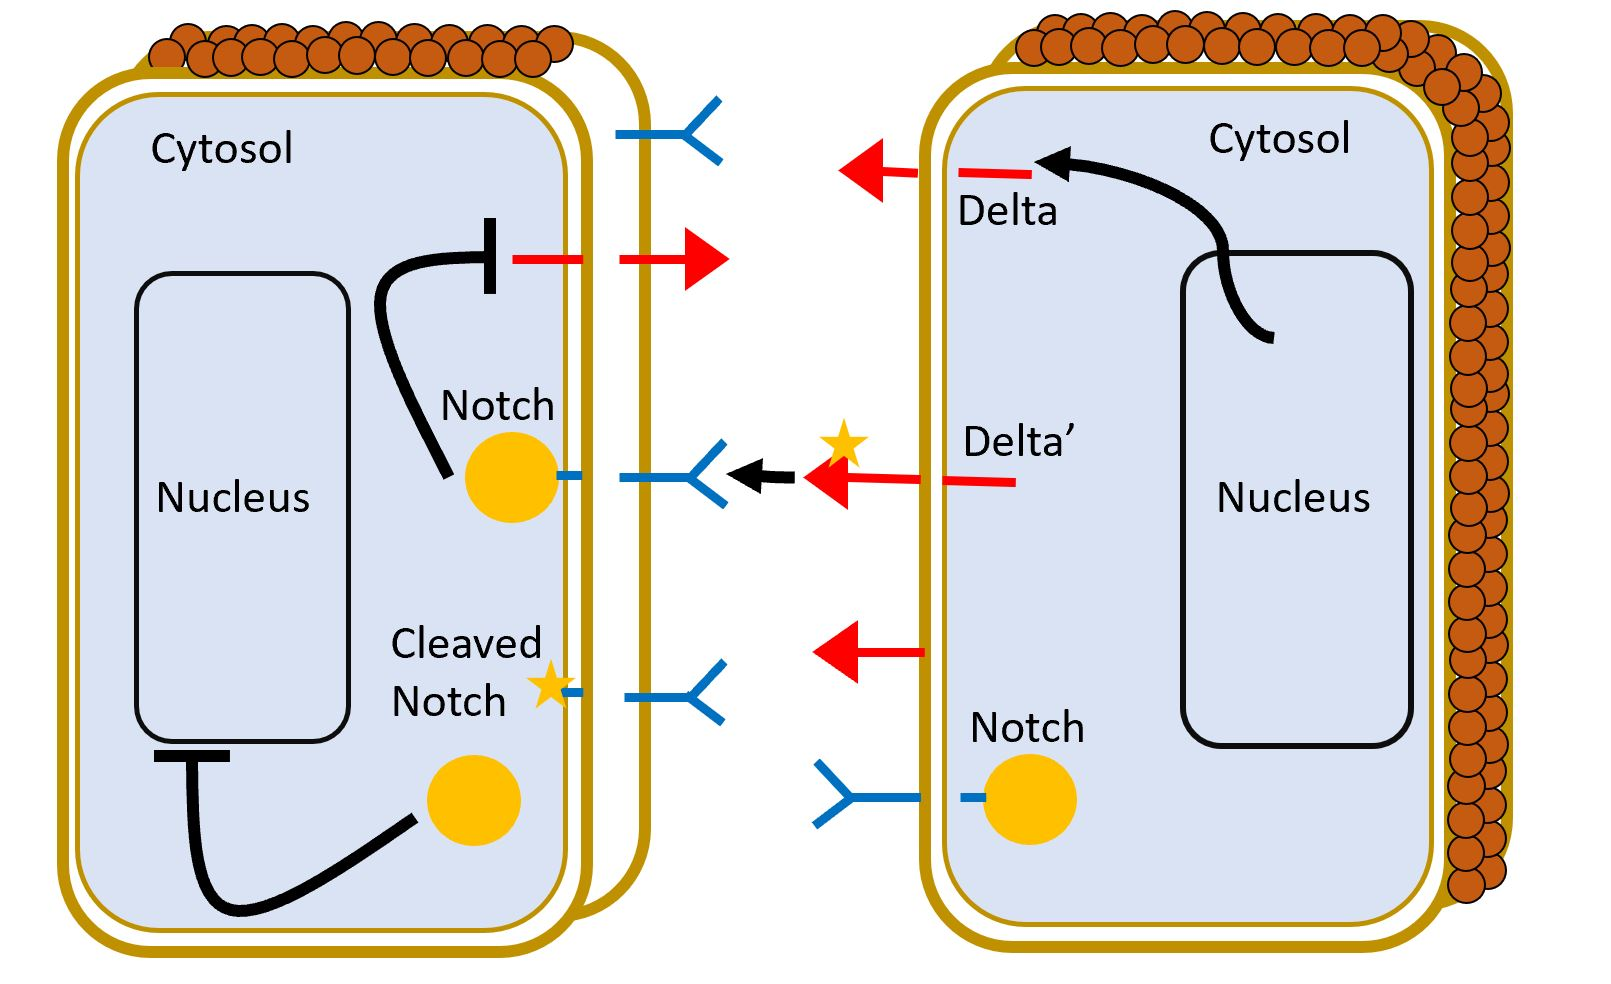
\includegraphics[width=8.4cm]{Overview_of_Delta_Notch}    % The printed column width is 8.4 cm.
\caption{Overview of the Delta-Notch Signaling pathway: Nucleus of the cells produce Delta and Notch membrane proteins. Delta protein is modeled to enter an activated Delta prime state according to Reynolds etc al. Delta Reacts with Notch, which leads to the cleavage of the internal region of Notch, which will then be known as Cleaved Notch or Nuclear Notch inside the nucleus in this paper. Subsequent repression or activation of cellular genes occurs once Nuclear Notch reaches the nucleus. Notch also represses expression and thus the activity of surrounding Delta membrane proteins, and eventual equilibrium will result in one cell over expressing Notch and the other cell expressing Delta. This leads to an oscillation of cell expression until the equilibrium is settled and cell fates are determined. } 
\label{fig:bifurcation}
\end{center}
\end{figure}


 \texttt{ifacconf}
\footnote{
This is the default for the provided class file.}




\section{Methodology}

The base for the agent based model was the \emph{Drosphilla} cell model developed by Reynolds etc al. This model builds upon the Delta-Notch signaling using the Syn-Notch circuits developed by Todo etc al. The circuits tested are \emph{Two Genotype Two Layer}, \emph{Two Genotype Three Layer}, \emph{One Genotype Contact Inhibition}, \emph{One Genotype Contact Inhibition Two Syn-Notch}. Two Layer was further modified to include the motion of the cells to introduce cell mobility into the model.

The basic model without modifications operates using agents to model the following components of Notch-Delta signaling: Neucleus of the cell, the Delta and Notch proteins, Cleaved Notch protein, Nuclear Cleaved Notch protein, Delta Prime, and membrane bound Delta and Notch proteins. Shown in Figure [FIGURE] is the basic operation procedure following Notch-Delta signaling. Nucleus agents are called Nucleus-Breed and are told to produce Notch-breed and Delta-Breed agents depending on the circuit, of which modifications for each circuit will be discussed in their subsections. These Notch-breed and Delta-breed agents are given a randomized direction and told to "diffuse" out in a straight line towards the modeled cell membrane. The cell membrane is modeled as Lipid-breed agents and are formed in rows of 6 in a hexagonal shape with the Nucleus-breed centered at the middle. As Notch-breed and Delta-breed agents approach the Lipid-breed agents Reynolds model asks the Lipid-breed agents and the Notch and Delta agents to come within 1 distance unit of each other. When the Notch and Delta agents have gotten close enough they will transition into Membrane Notch and Delta agents and their movement is constrained to move only laterally along Lipid agents. After a provided parameter time for transition Lipid Delta agents will transform into active Delta Prime agents and will continue to move along the hexagonal membrane lipids. the activity of the signaling occurs when a Notch membrane agent is next to a Delta prime membrane agent but on two opposite cells. A Notch prime is created as the "cleavage" event. The Cleaved notch is told to remain inside the cell just behind the membrane, and a Cleaved notch agent them moves towards the nucleus. once the Agent reaches a distance from the nucleus it converts into a nuclear Cleaved notch agent. 

Behavior of the expression of the cell is then added depending on the fate that levels of Nuclear Cleaved Notch agent determine. Each model circuit has conditions for when the genes will be activated depending on the level of cleaved notch, such as the color of the cell and expression of secondary notch pathways or cadherin genes. 

\subsection{Two Genotype -  Two Layer Circuit}

Non mobile:
Two genotype - Two layer circuit is modeled based of of the Todo etc al. circuit design seen in figure [FIGURE] A. Cell line agents were modeled by removing the abiltiy of to produce both Delta and Notch proteins at the same time. First A cells are chosen at random using NetLogo's random number selector and these cells will produce Delta, all other cells will produce Notch. The cells that produce delta agents and turn blue, where adjacent B cells that have membranes that neighbor the A cells will be signaled by them. When a Notch cleavage occurs in the B cells Nuclear Notch is formed, and when it passes a threshold the cell will turn green indicating the Delta from the A cells has signaled activity in the B cells. In addition to the modeled fluorescence, the B cells are given the ability to express cadherin according to the circuit. In the Two genotype Two layer circuit mobility was added into the cells to covert the static lattice used in the Reynolds paper. A random number generator again chooses  random cells, however not it tells each chosen cell to move in a random direction. The goal is to mimic primitive diffusion of cells among the medium. 

\subsection{Two Genotype - Three Layer Circuit}

The Three layer circuit with Two genotype is modeled based on the circuit design seen in figure [FIGURE] B. Cell line agents in the Two layer had either Notch or Delta functionality to denote difference in genotype, however in Three layer circuit modeling the cells retain full functionality of Notch-Delta signaling. The modification is Cell line A expresses Delta 1 and Notch 2 while Cell line b expresses Delta 2 and Notch 1. Delta 2 is not compatible with Notch 1 and likewise for Notch 2 and Delta 1. This creates a feedback after the initial Notch-Delta signal event where A cell's Delta 1 activate B cell's Notch 1, leading to cell fate C and activating the expression of both the green fluorescence and the expression of Delta 2. Delta 2 feeds back on the A cells that activated the B cell and binds the Notch 2 on the A cells surface. this leads to the third D cell fate which is modeled to flouresce pink to be consistent with Todo etc al circuit design. Mobility was not modeled in this circuit design however geometry was constrained to mimic the layering found in the experimental results from Todo. 


\subsection{Single Genotype - Single Notch Two Layer Circuit}

Single Two layer circuit is what the Reynolds paper developed and modeled. In single notch circuits both cells are of the same genotype, expressing both Notch and Delta. The result is a "tug of war" between the cells as differences in the rate of Notch and Delta production and location on the membrane lead to eventual imbalances which settles to eventually developing the two cell fates. One cell overexpressing Notch forces the cell fate of the other to express delta in excess, and eventually the fates are reinforced as notch inhibits delta expression and vice versa. random diffusion was modeled as discussed above to allow for these imbalances to arise, and the addition of the flouresence code to the model allowed for a direct comparison between Todo results for Two layer Single notch before cadherin agglomeration and Reynolds \emph{Drosophilla} cell sheet layout. The experiments were therefore verified as a control to ensure Reynolds code could accurately represent Todo's results before any major circuit modifications.

\subsection{Single Genotype - Double Notch Three Layer Circuit}

Single Genotype Three layer is an extension from the Reynolds \emph{Drosophilla} model taking inspiration from Todo's three layer circuit design. Initially cells are modeled to behave identically to a Two layer Single genotype contact inhibition model. After a set and variable parameter termed "Threshold" after an accumulation of Cleaved Notch from the Delta-Notch signaling passes this threshold the cell's begin expressing a second Delta-Notch pathway. The fates of the cell were determined based on three fates: no Cleaved notch is a blue neuron cell, only Cleaved notch from the first pathway is a endothelial cell as before, and presence of both Cleaved notch from the first pathway and Cleaved notch from the second pathway indicate a third unnamed line of new type 2 endothelial cells. The intention in this addition is to observe is additional Delta-Notch pathways lead to collapse of the "Rosette" patter observed in nature and modeled by Reynolds.







\begin{figure}
\begin{center}
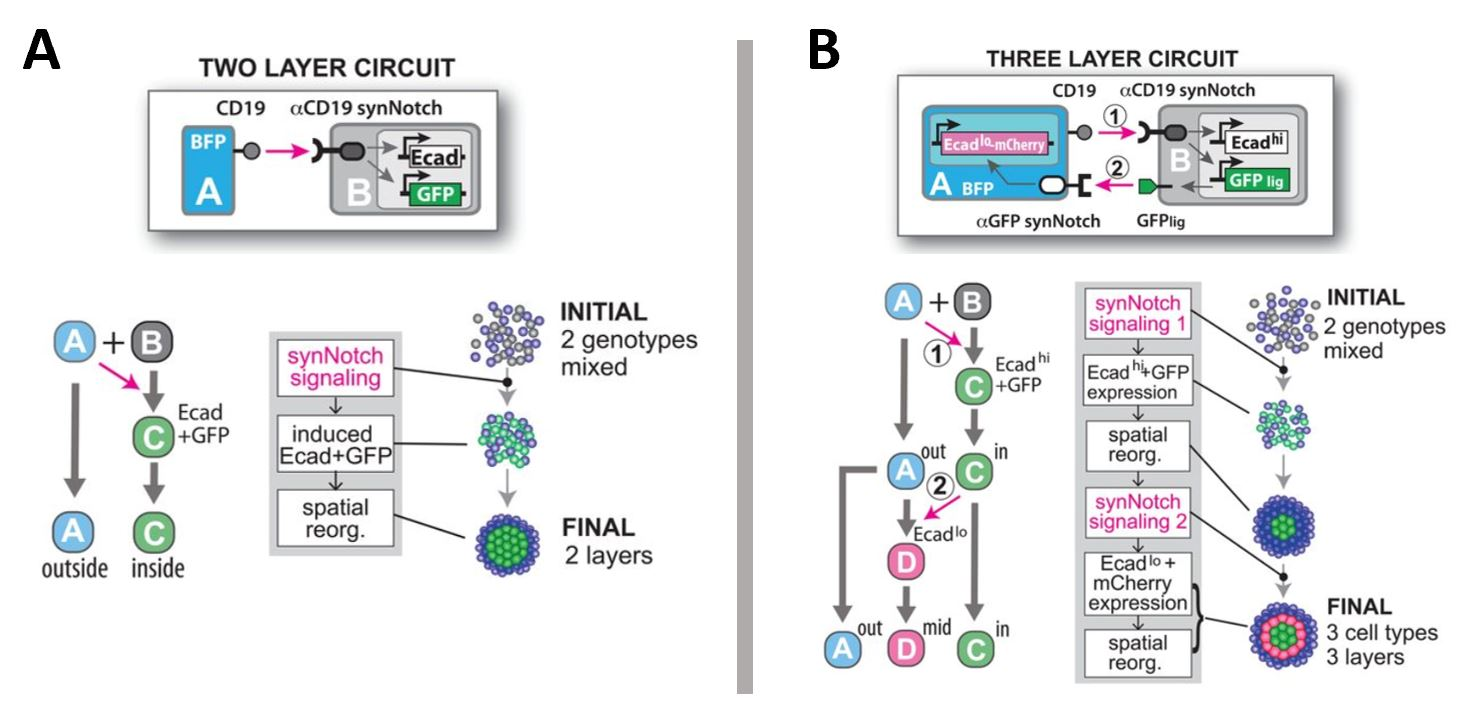
\includegraphics[width=8.4cm]{Todo_etc_al_layer_circuit_design}    % The printed column width is 8.4 cm.
\caption{Todo etc al. Two and Three layer Circuit of Syn- Notch: A) Two layer circuit design from Todo etc al where a mixture of two cell genotypes (A and B) are mixed and Syn-Notch signaling is allowed to occur. A cells activate B cells to turn into green C cells that will express cadherin which leads to agglomeration B) Three layer circuit design from Todo etc al where a mixture of two cell genotypes are mixed and Syn-Notch signaling occurs identical to the two later circuit. A second Syn-Notch pathway is added where activated C cells express Delta 2 which activates Notch 2 on A cells, which leads to the formation of the pink D cell line.  } 
\label{fig:bifurcation}
\end{center}
\end{figure}

\section{Results}

\subsection{Results for Two Genotype -  Two Layer Circuit} 

The Two layer Two genotype circuit operation can be seen in Figure [SOMETHINg] A. Initially a line of three identical cells are initiated in Netlogo. The Random selection is made, in this case it was set to select one third of the total cells available to be A cells. The A cell produced Delta alone as desired in the circuit and the delta interacted with the Notch on the neighboring black B cell. Cleaved notch can be seen accumulating just below the cell membrane of the now green C cell, which became a green cell after enough cleaved notch made it to the nucleus.

Mobility was then added to the cells, specific modifications are further explained according to appendix B to achieve the motion. from the figure [BLANK] in Appendix B cells were initially in the sheet as done before, and blue A cells and black B cells began moving around Netlogo agent space. As blue A cells reaches a radius close to B cells, the notch pathway activated as desired and many black cells became green B cells. Cadherin was programmed as a binary to save on computer resource, where activation of green fluorescence was also accompanied by cadherin activation. when two green B cells neared each other, and if both expressed Caherin they would slow down compared to other cells, leading to large "masses" of green cells surrounded mostly by individual blue neuron cells not attached to one another. 

\subsection{Results for Two Genotype - Three Layer Circuit} 

Three layer was constrained in its geometry, letting two rows of identical cells be generated to resemble a "Slice" of the balls of cells Todo generated.  Type A cells are again chosen at random, in the case of figure [SOMETHING] B a representative sample was chosen to highlight the proposed slice of the circle of cells. Blue A cells began producing Delta 1 and Notch 2 as desired, where black B cells were only producing Notch 1 as the color indicates. Activation proceeded according to Delta-Notch and the black B cells are now green C cells after an accumulation of Cleaved notch, indicated by the accumulation of cleaved notch just inside the yellow lipid membrane agents. Activation of the second Notch pathway (Delta 2 and Notch 2) is verified by the change of neighboring blue A cells turning pink, indicating the presence of Cleaved notch 2 and further identified by the layer of cleaved Notch 2 just behind the lipid membrane. The final layout resembles a 2 D slice of a circle of cells taken through the center.

\subsection{Results for Single Genotype - Single Notch Two Layer Circuit} 

Verification of the single genotype single notch circuit in the context of both Reynolds \emph{Drosophilla} cells and early random scattering of cells in Todo etc al. was able to both verify the "Rosette" pattering seen in Reynolds when left to reach equilibrium, while early patterns have features of Todo etc al scattering of cells before cadherin. In figure [something] A the formation of the Rosettes occurs only after reaching an equilibrium, where prior the cycling between one cell fate and the other, a key feature of Delta-Notch signaling, occurs and matches the initial stages of Todo circuits. The pattering is potentially a feature of the geometry of the system and inherent in Notch-Delta signaling, where the additional cadherin component of Toda circuits lead to the loss of Rosettes and formation of the clustering. 

\subsection{Results for Single Genotype - Double Notch Three Layer Circuit} 

To examine if rosette formation could be interrupted by the addition of the second Syn-Notch pathway the model was run and figure [blacnk] B shows the new equilibrium state of the three layer circuit. Notable features of the new cell layout is that "Rosette" formation appears to follow a new geometry. Neuron cells, and two types of endothelial cells are present. Neurons are surrounded by both green an pink cell lines in two unique formations. One layout is a blue neuron cell with two pink cells on the left and two on the right with one Green cell above and one green cell below the neuron. the second new layout is the neuron surrounded by green and pink cells, where cells alternate in color as it goes around the neuron. Rosette pattering was retained according to the original definition, in that a single neuron cell is surrounded by cells of endothelial lineage. 











\begin{figure}
\begin{center}
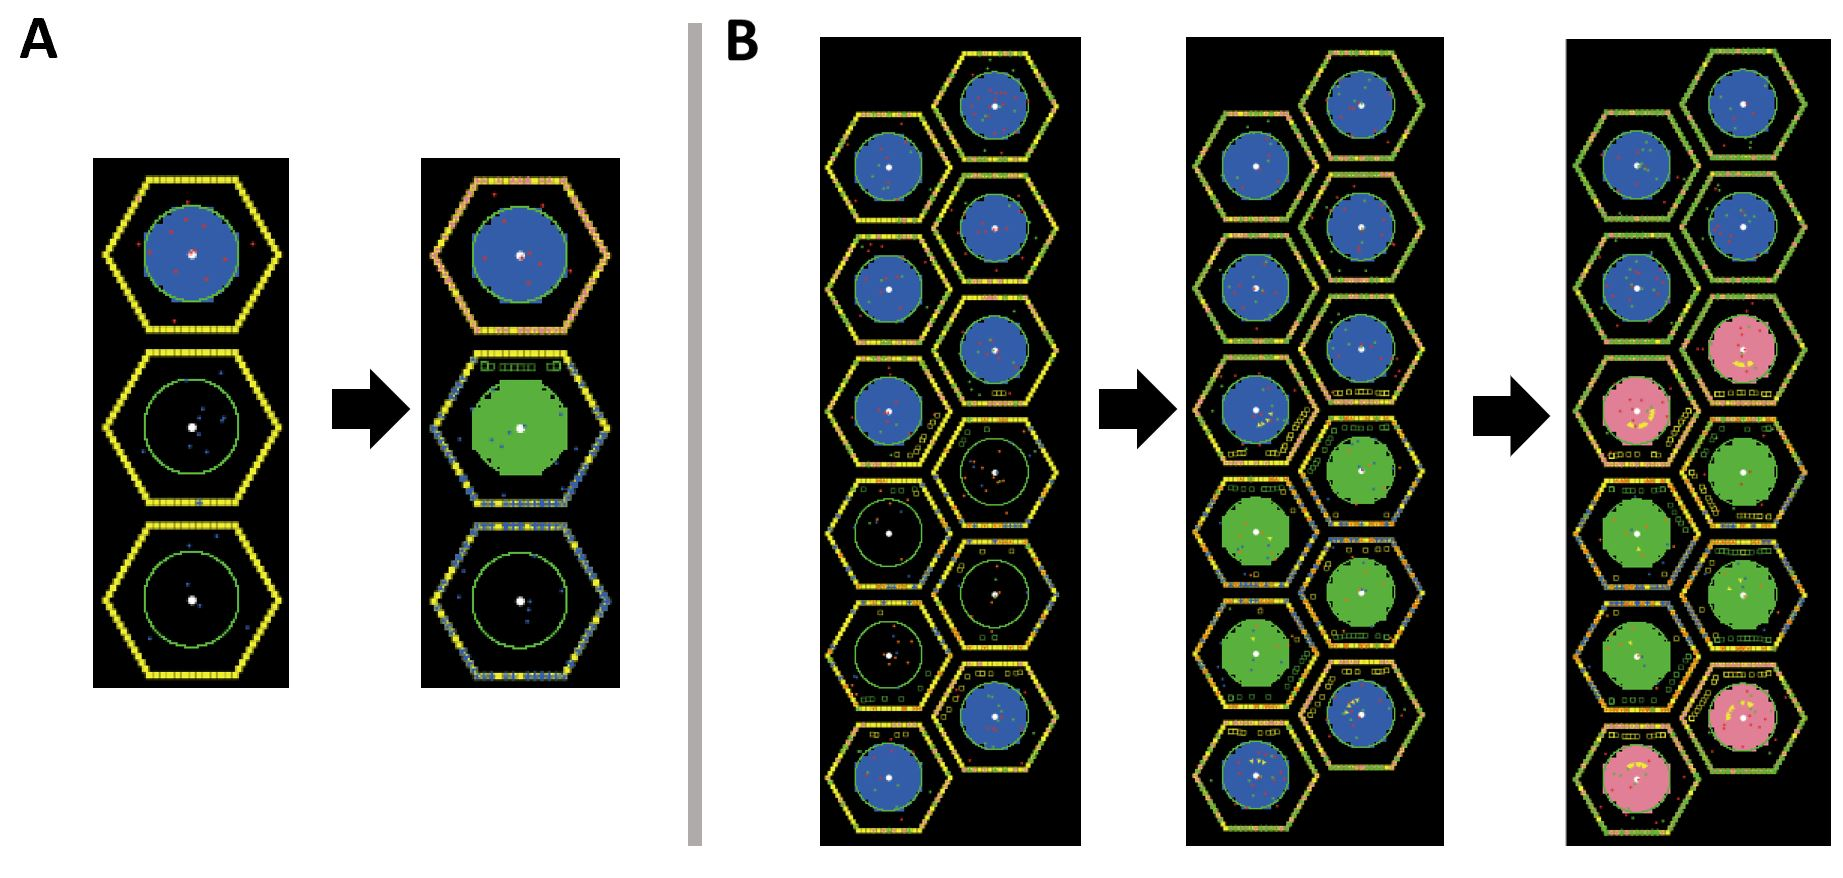
\includegraphics[width=8.4cm]{Two_and_Three_layer_Two_Genotype}    % The printed column width is 8.4 cm.
\caption{Two and Three layer Circuit of Syn- Notch: A) Starting cells are initially allowed to produce either Notch or Delta where Delta producing cells are labeled blue. After time has passed cells expressing Notch have been activated by neighboring blue cells and will turn green. If there are no neighboring cells the Notch expressing cells will remain black. B) Three layer circuit where blue cells are chosen to express Delta and Notch 2. Neighboring cells expressing Notch are activated and turn green and will begin expressing Delta 2. Neighboring blue cells are then activated by green cells' Delta 2 which causes blue cells to turn pink. result is a striped layer structure.  } 
\label{fig:bifurcation}
\end{center}
\end{figure}

\begin{figure}
\begin{center}
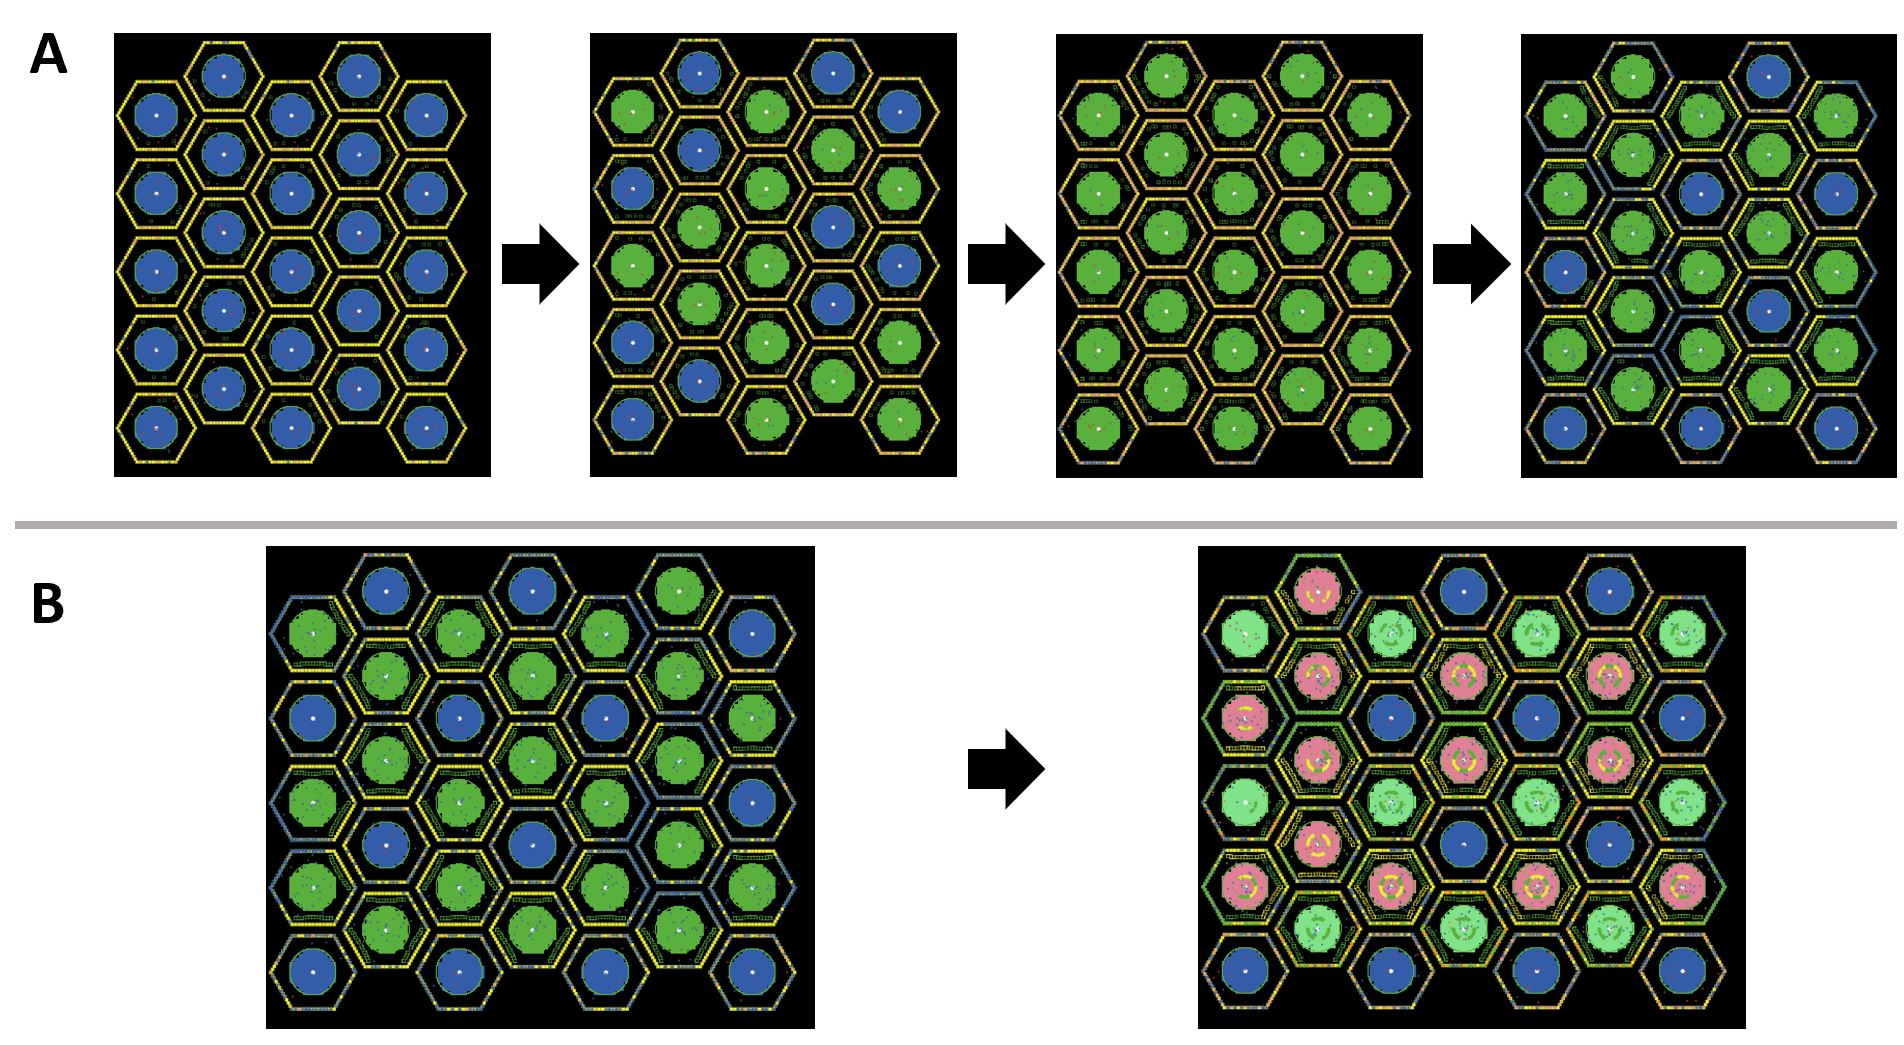
\includegraphics[width=8.4cm]{One_Genotype_two_and_one_SynNotch}    % The printed column width is 8.4 cm.
\caption{Two layer Circuit of Syn- Notch Single Genotype: A) One genotype Delta-Notch signaling replication of \emph{Drosophilla} seen in Reynolds etc al. Cells start of as neurons producing both Notch and Delta, leading to the "tug of war" beteen the cell fates seen as it alternates between all blue and all green cell lines. Eventually an equilibrium is reached which holds the "Rosette" patterns characteristic in \emph{Drosophilla} cell development.  B) The cell sheet on the left is the single Notch-Delta circuit. The right is the change in equilibrium layout after the addition of the second Syn-Notch pathway. Rosettes are now complex combinations of endothelial cells (green and pink) surrounding the central Neuron (blue) cells. } 
\label{fig:bifurcation}
\end{center}
\end{figure}



See \cite{Abl:56}, \cite{AbTaRu:54}, \cite{Keo:58} and \cite{Pow:85}.



\begin{thm}   % use the thm environment for theorems
The square of the length of the hypotenuse of a right triangle equals
the sum of the squares of the lengths of the other two sides.
\end{thm}

\begin{pf}    % and the pf environment for proofs
The square of the length of the hypotenuse of a right triangle equals the sum of the squares 
of the lengths of the other two sides.
\end{pf}

%% There are a number of predefined theorem-like environments in
%% ifacconf.cls:
%%
%% \begin{thm} ... \end{thm}            % Theorem
%% \begin{lem} ... \end{lem}            % Lemma
%% \begin{claim} ... \end{claim}        % Claim
%% \begin{conj} ... \end{conj}          % Conjecture
%% \begin{cor} ... \end{cor}            % Corollary
%% \begin{fact} ... \end{fact}          % Fact
%% \begin{hypo} ... \end{hypo}          % Hypothesis
%% \begin{prop} ... \end{prop}          % Proposition
%% \begin{crit} ... \end{crit}          % Criterion

Of course LaTeX manages equations through built-in macros. You may
wish to use the \texttt{amstex} package for enhanced math
capabilities.

Figures must be centered, and have a caption at the bottom. 

\subsection{Tables}
Tables must be centered and have a caption above them, numbered with
Arabic numerals. See table~\ref{tb:margins} for an example.

\begin{table}[hb]
\begin{center}
\caption{Margin settings}\label{tb:margins}
\begin{tabular}{cccc}
Page & Top & Bottom & Left/Right \\\hline
First & 3.5 & 2.5 & 1.5 \\
Rest & 2.5 & 2.5 & 1.5 \\ \hline
\end{tabular}
\end{center}
\end{table}

\subsection{Final Stage}

Authors are expected to mind the margins diligently.  Papers need to
be stamped with event data and paginated for inclusion in the
proceedings. If your manuscript bleeds into margins, you will be
required to resubmit and delay the proceedings preparation in the
process.

\subsubsection{Page margins.} See table~\ref{tb:margins} for the
page margins specification. All dimensions are in \emph{centimeters}.


\subsection{PDF Creation}

All fonts must be embedded/subsetted in the PDF file. Use one of the
following tools to produce a good quality PDF file:

\subsubsection{PDFLaTeX} is a special version of LaTeX by Han The
Thanh which produces PDF output directly using Type-1 fonts instead of
the standard \texttt{dvi} file. It accepts figures in JPEG, PNG, and PDF
formats, but not PostScript. Encapsulated PostScript figures can be
converted to PDF with the \texttt{epstopdf} tool or with Adobe Acrobat
Distiller.

\subsubsection{Generating PDF from PostScript} is the classical way of
producing PDF files from LaTeX. The steps are:

\begin{enumerate}
  \item Produce a \texttt{dvi} file by running \texttt{latex} twice.
  \item Produce a PostScript (\texttt{ps}) file with \texttt{dvips}.
  \item Produce a PDF file with \texttt{ps2pdf} or Adobe Acrobat
  Distiller.
\end{enumerate}

\subsection{Copyright Form}

IFAC will put in place an electronic copyright transfer system in due
course. Please \emph{do not} send copyright forms by mail or fax. More
information on this will be made available on IFAC website.


\section{Units}

Use SI as primary units. Other units may be used as secondary units
(in parentheses). This applies to papers in data storage. For example,
write ``$15\,\mathrm{Gb}/\mathrm{cm}^2$ ($100\,\mathrm{Gb}/\mathrm{in}^2$)''. 
An exception is when
English units are used as identifiers in trade, such as ``3.5 in
disk drive''. Avoid combining SI and other units, such as current in
amperes and magnetic field in oersteds. This often leads to confusion
because equations do not balance dimensionally. If you must use mixed
units, clearly state the units for each quantity in an equation.  The
SI unit for magnetic field strength $\mathbf{H}$ is $\mathrm{A}/\mathrm{m}$. However, if you wish to
use units of $\mathrm{T}$, either refer to magnetic flux density $\mathbf{B}$ or
magnetic field strength symbolized as $\mu_0\,\mathbf{H}$. Use the center dot to
separate compound units, e.g., ``$\mathrm{A} \cdot \mathrm{m}^2$''.

\section{Helpful Hints}

\subsection{Figures and Tables}

Figure axis labels are often a source of confusion. Use words rather
than symbols. As an example, write the quantity ``Magnetization'', or
``Magnetization M'', not just ``M''. Put units in parentheses. Do not
label axes only with units.  For example, write ``Magnetization
($\mathrm{A}/\mathrm{m}$)'' or ``Magnetization ($\mathrm{A} \mathrm{m}^{-1}$)'', not just
 ``$\mathrm{A}/\mathrm{m}$''. Do not
label axes with a ratio of quantities and units. For example, write
``Temperature ($\mathrm{K}$)'', not ``$\mbox{Temperature}/\mathrm{K}$''.

Multipliers can be especially confusing. Write ``Magnetization
($\mathrm{kA}/\mathrm{m}$)'' or ``Magnetization ($10^3 \mathrm{A}/\mathrm{m}$)''. Do not write
``Magnetization $(\mathrm{A}/\mathrm{m}) \times 1000$'' because the reader would not know
whether the axis label means $16000\,\mathrm{A}/\mathrm{m}$ or $0.016\,\mathrm{A}/\mathrm{m}$.

\subsection{References}

Use Harvard style references (see at the end of this document). With
\LaTeX, you can process an external bibliography database 
using \texttt{bibtex},\footnote{In this case you will also need the \texttt{ifacconf.bst}
file, which is part of the \texttt{ifaconf} package.}
or insert it directly into the reference section. Footnotes should be avoided as
far as possible.  Please note that the references at the end of this
document are in the preferred referencing style. Papers that have not
been published should be cited as ``unpublished''.  Capitalize only the
first word in a paper title, except for proper nouns and element
symbols.

\subsection{Abbreviations and Acronyms}

Define abbreviations and acronyms the first time they are used in the
text, even after they have already been defined in the
abstract. Abbreviations such as IFAC, SI, ac, and dc do not have to be
defined. Abbreviations that incorporate periods should not have
spaces: write ``C.N.R.S.'', not ``C. N. R. S.'' Do not use abbreviations
in the title unless they are unavoidable (for example, ``IFAC'' in the
title of this article).

\subsection{Equations}

Number equations consecutively with equation numbers in parentheses
flush with the right margin, as in (\ref{eq:sample}).  To make your equations more
compact, you may use the solidus ($/$), the $\exp$ function, or
appropriate exponents. Use parentheses to avoid ambiguities in
denominators. Punctuate equations when they are part of a sentence, as
in

\begin{equation} \label{eq:sample2}
\begin{array}{ll}
\int_0^{r_2} & F (r, \varphi ) dr d\varphi = [\sigma r_2 / (2 \mu_0 )] \\
& \cdot \int_0^{\inf} exp(-\lambda |z_j - z_i |) \lambda^{-1} J_1 (\lambda  r_2 ) J_0 (\lambda r_i ) d\lambda 
\end{array}
\end{equation}

Be sure that the symbols in your equation have been defined before the
equation appears or immediately following. Italicize symbols ($T$
might refer to temperature, but T is the unit tesla). Refer to
``(\ref{eq:sample})'', not ``Eq. (\ref{eq:sample})'' or ``equation
(\ref{eq:sample})'', except at the beginning of a sentence: ``Equation
(\ref{eq:sample}) is \ldots''.

\subsection{Other Recommendations}

Use one space after periods and colons. Hyphenate complex modifiers:
``zero-field-cooled magnetization''. Avoid dangling participles, such
as, ``Using (1), the potential was calculated'' (it is not clear who or
what used (1)). Write instead: ``The potential was calculated by using
(1)'', or ``Using (1), we calculated the potential''.

A parenthetical statement at the end of a sentence is punctuated
outside of the closing parenthesis (like this). (A parenthetical
sentence is punctuated within the parentheses.) Avoid contractions;
for example, write ``do not'' instead of ``don' t''. The serial comma
is preferred: ``A, B, and C'' instead of ``A, B and C''.


\section{Conclusion}

A conclusion section is not required. Although a conclusion may review
the main points of the paper, do not replicate the abstract as the
conclusion. A conclusion might elaborate on the importance of the work
or suggest applications and extensions.

\begin{ack}
Place acknowledgments here.
\end{ack}

\bibliography{ifacconf}             % bib file to produce the bibliography
                                                     % with bibtex (preferred)
                                                   
%\begin{thebibliography}{xx}  % you can also add the bibliography by hand

%\bibitem[Able(1956)]{Abl:56}
%B.C. Able.
%\newblock Nucleic acid content of microscope.
%\newblock \emph{Nature}, 135:\penalty0 7--9, 1956.

%\bibitem[Able et~al.(1954)Able, Tagg, and Rush]{AbTaRu:54}
%B.C. Able, R.A. Tagg, and M.~Rush.
%\newblock Enzyme-catalyzed cellular transanimations.
%\newblock In A.F. Round, editor, \emph{Advances in Enzymology}, volume~2, pages
%  125--247. Academic Press, New York, 3rd edition, 1954.

%\bibitem[Keohane(1958)]{Keo:58}
%R.~Keohane.
%\newblock \emph{Power and Interdependence: World Politics in Transitions}.
%\newblock Little, Brown \& Co., Boston, 1958.

%\bibitem[Powers(1985)]{Pow:85}
%T.~Powers.
%\newblock Is there a way out?
%\newblock \emph{Harpers}, pages 35--47, June 1985.

%\bibitem[Soukhanov(1992)]{Heritage:92}
%A.~H. Soukhanov, editor.
%\newblock \emph{{The American Heritage. Dictionary of the American Language}}.
%\newblock Houghton Mifflin Company, 1992.

%\end{thebibliography}

\appendix
\section{A summary of Latin grammar}    % Each appendix must have a short title.
\section{Some Latin vocabulary}              % Sections and subsections are supported  
                                                                         % in the appendices.
\end{document}
